\documentclass{article}
\usepackage{amsmath, amsfonts}
\usepackage{tikz}
\usepackage{pgfplots}

\begin{document}

\title{Exact Sampling}
\author{Sebastian Oberhoff}

\maketitle

\begin{abstract}
It is a widely accepted truism that anytime computers come into contact with real numbers some numerical inaccuracy must be incurred. In this article we'll see an exception to this rule in the arena of random sampling. In particular, we'll discover that irrational probabilities pose almost no obstacle towards exact sampling at all.

Furthermore, we'll see that even if our \textit{samples} are irrational, as they are in the case of continuous distributions, we can still make remarkable headway by extracting finite \textit{prefixes} that fully characterize the sought distribution.
\end{abstract}


\noindent
\section{Introduction}

Imagine we had access to an infinite supply of independent random bits equally likely to be 0 or 1, for instance by flipping a coin. And suppose we were asked to simulate a weighted random bit with probability $p=0.25$ for 0 and 0.75 for 1. Using the infinite supply of bits at our command this is a straightforward task. Simply map the first two bits as follows:
\[
\begin{split}
00 \rightarrow 0\\
01 \rightarrow 1\\
10 \rightarrow 1\\
11 \rightarrow 1
\end{split}
\]
This much is easy. But what if $p$ was a more complicated number such as $1/\pi$? This seems like a much more challenging task. Indeed, here is a "proof" that it is impossible to perform this task exactly.

Any finite computation can only examine a finite number, say $n$, of the input bits. This sequence of $n$ input bits takes on every possible value with equal probability of $2^{-n}$. No matter what computation we perform on this sequence, ultimately 0 will result with some probability that is a multiple of $2^{-n}$. But $1/\pi$ isn't a multiple of $2^{-n}$ for any $n$. Even though we can make the error arbitrarily small, some will always remain.

This argument seems very persuasive. And yet there is a loophole. Consider the following procedure.

First, try thinking of the infinite sequence of random bits we have access to as an exact sample from the uniform distribution on the interval $[0,1]$, which has been given in binary. This sample falls below $1/\pi$ with probability $1/\pi$ exactly. But how do we compare two infinitely long sequences of digits? Here's how: Begin by writing out a few digits of the binary representation of $1/\pi$.
$$\frac{1}{\pi} = 0.0101000101..._2$$
Then compare the bits beyond the decimal point with the random bits $b_i$ we've been given.
\[
\begin{matrix}
0 & 1 & 0 & 1 & 0 & 0 & 0 & 1 & 0 & 1\\
\updownarrow & \updownarrow & \updownarrow & \updownarrow & \updownarrow & \updownarrow & \updownarrow & \updownarrow & \updownarrow & \updownarrow \\
b_0 & b_1 & b_2 & b_3 & b_4 & b_5 & b_6 & b_7 & b_8 & b_9
\end{matrix}
\]
If all of these bits miraculously agree with each other, just compute some more bits of $1/\pi$ and compare these with more random bits. Sooner or later we'll find a disagreement between these two sequences. At that point we know which is larger, the rest of the infinite sequence of bits of either number doesn't matter!

We'll refer to this trick, originating as far as I'm aware from \cite{Knuth-Yao}, as \textit{exact Bernoulli sampling}. It circumvents the "proof" given earlier by potentially running arbitrarily long. And yet it is by no means infeasible. The number of required comparisons follows a geometric distribution with $p=1/2$, so the expected number of required comparisons is a mere 2. Also note that we didn't depend in any way on special properties of $1/\pi$. We could have proceeded in the same way with any computable number imaginable as our $p$. The only component that can cause worry is the complexity of computing digits of $p$, though we won't meet any examples where this becomes a critical issue here. The plan for the rest of this discussion is to take exact Bernoulli sampling and milk it as much as possible.

\section{Exact Discrete Sampling}

\subsection{Exact Bisection Sampling}

Say our next challenge was to draw exact samples from the Poisson distribution with parameter $\lambda = 5$. Here's how we could do it. First, we find a rational number that is close to the median. (Using rationals just makes the procedure simpler.) As Figure \ref{fig:bisection_0} demonstrates, using 4.5 as our midpoint will do nicely.

\pgfmathdeclarefunction{poiss}{1}{%
	\pgfmathparse{(#1^x)*exp(-#1)/(x!)}%
}

\begin{figure}[h]
	\centering
	\begin{tikzpicture}[scale=1.3]
	\begin{axis}[tick label style={/pgf/number format/fixed}, every axis plot post/.append style={
		samples at = {0,...,15},
		axis x line*=bottom,
		axis y line*=left,
		enlargelimits=upper}]
	\addplot +[ycomb] {poiss(5)};
	\draw[red, very thick] (45, 0) -- (45, 200);
	\end{axis}
	\end{tikzpicture}
	\caption{Approximate bisection of the Poisson distribution with $\lambda = 5$ using 4.5 as the mid point}
	\label{fig:bisection_0}
\end{figure}

We can then compute the probability that any sample will fall on the left side of this line by computing the leading bits of the cumulative distribution function at 4.5.
$$F(4.5) = 0.0111000011..._2$$
where $F$ is the distribution function of the Poisson distribution with $\lambda = 5$. Using a few of these bits together with exact Bernoulli sampling we can now determine which way to proceed with our search.

For the purpose of illustration, let's assume that our first bisection led us to the right. We then rescale our probabilities by conditioning on the fact that our sample is greater than 4.5 and bisect this new probability distribution as in Figure \ref{fig:bisection_1}.

\begin{figure}[h]
	\centering
	\begin{tikzpicture}[scale=1.3]
	\begin{axis}[every axis plot post/.append style={
		samples at = {5,...,20},
		axis x line*=bottom,
		axis y line*=left,
		enlargelimits=upper}]
	\addplot +[ycomb] {poiss(5)/0.5595};
	\draw[red, very thick] (15, 0) -- (15, 350);
	\end{axis}
	\end{tikzpicture}
	\caption{Approximately bisect the Poisson distribution above 4.5 using 6.5 as the new mid point}
	\label{fig:bisection_1}
\end{figure}

At this point the idea should be clear. Keep bisecting the remaining range until only a single integer is the sole remaining possibility. That will then be our sample. As long as we don't choose our mid points in a completely silly fashion the number of steps we'll be walking off to the right will follow an approximately geometric distribution. And as soon as we turn back around we'll terminate very soon after.

Of course, none of these considerations were very particular to the Poisson distribution with $\lambda = 5$. So this method is evidently applicable to virtually any discrete distribution one could care to name.

\subsection{Exact Discrete Inverse Sampling}

Another procedure that is in many respects quite similar can be constructed from inverse sampling. That is, if $X \sim \text{U}[0,1]$, then $F^{-1}(X)$ will be distributed according to the Poisson distribution with $\lambda = 5$ \footnote{to be exact $F^{-1}$ must be defined to return the smallest $n \in \mathbb{N}$ such that $F(n) \geq X$ (we use the convention that $\mathbb{N}$ includes 0)}. One way to visually represent this is by labeling the unit interval as in Figure \ref{fig:inverse}. Then we drop a sample $X$ onto the line, observe which interval the sample fell in, and choose the next largest corresponding $n$ as our sample.

\begin{figure}[t!]
	\centering
	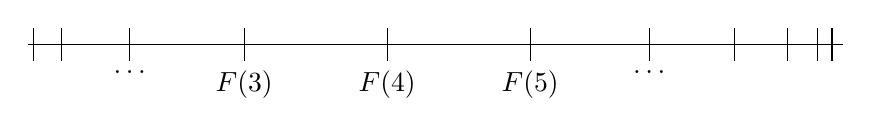
\begin{tikzpicture}[scale=0.03\textwidth]
	\draw (0,0) -- (1,0);
	\draw (0.0067, -0.02) -- (0.0067, 0.02);
	\draw (0.0404, -0.02) -- (0.0404, 0.02);
	\draw (0.1246, -0.02) node[below]{$\hdots$}
	-- (0.1246, 0.02);
	\draw (0.2650, -0.02) node[below]{$F(3)$}
	-- (0.2650, 0.02);
	\draw (0.4404, -0.02) node[below]{$F(4)$}
	-- (0.4404, 0.02);
	\draw (0.6159, -0.02) node[below]{$F(5)$}
	-- (0.6159, 0.02);
	\draw (0.7621, -0.02) node[below]{$\hdots$}
	-- (0.7621, 0.02);
	\draw (0.8666, -0.02) -- (0.8666, 0.02);
	\draw (0.9319, -0.02) -- (0.9319, 0.02);
	\draw (0.9681, -0.02) -- (0.9681, 0.02);
	\draw (0.9863, -0.02) -- (0.9863, 0.02);
	\end{tikzpicture}
	\caption{The unit interval divided into sections according to the Poisson distribution function when $\lambda = 5$}
	\label{fig:inverse}
\end{figure}

We can easily make this procedure exact by sampling the digits of $X$ one by one and computing the leading digits of $F$ for the various relevant values of $n$. Eventually we'll have $X$ completely fenced in between $F(n)$ and $F(n+1)$ for some $n$, at which point none of the remaining digits of any of the involved quantities matter, so we can return $n+1$.

\section{Exact Rejection Sampling}

Finally, we'll turn our attention to continuous distributions. Immediately a problem presents itself here. That is, a sample from a continuous distribution will typically be an irrational number with infinitely many digits in its decimal representation. How can we hope to draw an exact sample if just printing it out is an indeterminate process?\\
Clearly, we'll have to manage our expectations as to what we can accomplish here. But if all we ask for is a method that will produce arbitrarily many correct digits of an exact sample, then the standard toolbox already provides plenty of options.

Take the inverse sampling method again. In the case of the exponential distribution with $\lambda = 1$ this method amounts to simply computing $-\ln(1-X)$ where $X \sim \text{U}[0,1]$. This task can be performed to arbitrary precision. So in the sense just described exact sampling would be quite uninteresting.

But there's another sense in which exact sampling can be accomplished which isn't quite as trivial. We can try to sample just the leading digits of an exact sample so that the remaining digits then no longer depend on the distribution we're sampling from. In particular we'll see a way to sample leading digits, which we'll call a prefix, so that the remaining digits will be uniformly random. A prefix thus completely captures the characteristics of the distribution and so can arguably be referred to as an exact sample.

The tool we'll use to accomplish this is a modification of \textit{rejection sampling}. The method of rejection sampling goes back to John von Neumann and is probably easiest to understand from a visual perspective. The idea is to graph the density $f$ of the desired target distribution and throw uniformly random darts at the area below $f$. How does one throw these uniformly random darts? By throwing uniformly random darts at an enclosing area until a dart hits the target area. Darts that miss are rejected---hence the name rejection sampling. The advantage is that, whereas it might not be clear how to generate uniform samples in the area below $f$, the enclosing area might be simpler. For example one can always just use a simple rectangle as the enclosing area. And a uniform sample from a rectangle is built simply from two independent uniform samples $x$ and $y$ which, luckily, is just what we have readily available.

\begin{figure}
	\centering
	\begin{tikzpicture}[scale=1.3]
	\begin{axis}
	\path[fill=gray!15] (0, 0) -- (100, 0) -- (100, 200) -- cycle;
	\addplot[mark=none,very thick,color=blue] coordinates {(0, 0) (1, 2)};
	\node[circle,fill=red,scale=0.5] at (60, 70) {};
	\end{axis}
	\end{tikzpicture}
	\caption{Rejection Sampling --- Samples that fall in the shaded region (as shown) are accepted}
	\label{fig:rejection_0}
\end{figure}

As an example, let our target distribution be the distribution with density
\[
f(x)=
\begin{cases}
2x & 0 \leq x < 1\\
0 & \text{otherwise}
\end{cases}\,.
\]
Rejection sampling then says to do the following:
\begin{enumerate}
	\item Draw a uniform sample $(x, y)$ from U$[0,1]\times[0,2]$
	\item Accept $x$ as the sample if $y \leq 2x$
	\item If $x$ was rejected, start over
\end{enumerate}
These steps can be visualized as in Figure \ref{fig:rejection_0}.

The way this is usually implemented is by approximating the uniform distribution using some finite number of bits, inevitably incurring some error. But using exact Bernoulli sampling we can do better.

In essence, we'll consider the rectangle defined by the leading digits of $x$ and $y$. By drawing additional digits for $x$ and $y$ we can shrink this rectangle arbitrarily small until we're certain that it falls either wholly below or above $f$. At that point we know whether to accept or reject, without having to examine further digits. Let's walk through an example.

Suppose the leading bits of our uniform sample $x$ are $101...\,.$ This narrows down our sample to the interval [0.625, 0.75]. We can think of this as defining a $\delta$-environment from basic calculus. This in turn defines a corresponding $\epsilon$-environment [1.25, 1.5] into which $f(x)=2x$ falls.

Furthermore, let's imagine that the leading bits of our second sample $y$, drawn from U[0, 2], were $1001...\,.$ This allows us to narrow down $y$ to [1.125, 1.375]. Figure \ref{fig:rejection_1} shows what's going on.

\begin{figure}[h]
	\centering
	\begin{tikzpicture}[scale=1.3]
	\begin{axis}
	\path[fill=gray!15] (10, 137.5) -- (90, 137.5) -- (90, 150) -- (10, 150);
	
	\path[fill=gray!30] (20, 125) -- (90, 125) -- (90, 137.5) -- (20, 137.5);
	
	\path[fill=gray!15] (10, 125) -- (20, 125) -- (20, 137.5) -- (10, 137.5);
	
	\path[fill=gray!15] (90, 125) -- (100, 125) -- (100, 137.5) -- (90, 137.5);
	
	\path[fill=gray!15] (20, 112.5) -- (100, 112.5) -- (100, 125) -- (20, 125);
	
	\addplot[mark=none,very thick, color=blue] coordinates {(0, 0) (1, 2)};
	
	\draw[dashed] (62.5, 0) -- (62.5, 200);
	\draw[dashed] (75, 0) -- (75, 200);
	
	\draw[dashed] (10, 150) -- (90, 150);
	\draw[dashed] (10, 125) -- (90, 125);
	
	\draw[dashed] (20, 137.5) -- (100, 137.5);
	\draw[dashed] (20, 112.5) -- (100, 112.5);
	
	\draw[decoration={brace, mirror}, decorate] (101, 112.5) -- node[right] {$y$} (101, 137.5);
	
	\draw[decoration={brace}, decorate] (9, 125) -- node[left] {$f(x)$} (9, 150);
	
	\draw[decoration={brace, mirror}, decorate] (62.5, -1) -- node[below] {$x$} (75, -1);
	\end{axis}
	\end{tikzpicture}
	\caption{Having drawn $x = 0.101..._2$ and $y = 1.001..._2$ we know that $x$, $y$, and $f(x)$ fall somewhere into these intervals}
	\label{fig:rejection_1}
\end{figure}

Now these intervals for $f(x)$ and $y$ overlap. So we can't say for certain whether $x$ should be rejected or not. But that's easy to remedy. Just draw additional bits for $x$ and $y$. Sooner or later (and chances are sooner) these intervals will separate. And then we'll know whether to accept $x$ or to try again.

But note that something remarkable happens as soon as we accept $x$. At that point we've determined some of the leading bits of $x$ through careful testing with the rejection method. But the remaining bits can now be drawn from our infinite random bit supply without any further thought! We can forget all about the function $f(x)=2x$ and just pump out the remaining bits of our sample as fast as our random number generator is able to mint them.

\section{Putting It All Together}

Now let's take these two previous ideas and put them together. How could we draw an exact sample from the standard normal distribution? At this point it's simple. First, use exact bisection sampling and perform a random walk on the integers, starting at 0. As soon as the sample has been narrowed down to an interval of unit length, the integer part of the sample has been determined. Then use exact rejection sampling to determine the fractional part. That's all there is to it. We can now easily produce the digits of an exactly standard normally distributed sample to our hearts content.

\section{A Bird's Eye View}

At this point it seems worth reflecting a little more generally. First, let's direct our attention to the bits required to sample $x$ during the rejection sampling stage. A few of these bits will be discarded while we iterate the rejection method. But the rest is then returned completely unmodified. A different way of looking at this is that we're taking a sample from the uniform distribution and sawing off a little piece at the front. The tail end is then precisely the fractional part of a random variable having practically any desired continuous distribution.

Furthermore, we could have used the exact same sequence to also draw an exact sample from some other unrelated distribution. These two samples would then be correlated in the curious way that, at some offset, eventually all of their digits coincide. Stated differently, if one looks at a sample from the uniform distribution, chances are that, \textit{within eyesight}, one can see the superimposed beginnings of samples from any continuous distribution one can care to mention.

Also, consider the following. After having determined the leading digits of a sample from some distribution, we could write them down on a slip of paper and pass it to somebody else. We'll call such string of digits a \textit{prefix}. That person wouldn't even have to know which distribution the prefix was drawn from. They would still hold in their hands an \textit{exact} sample. If they're unsatisfied with the precision of the prefix we gave them, they can just add their own random digits! Reminiscent of the way that the symbol $\pi$ summarizes an infinite sequence of digits, so do the digits on that slip of paper.

As an aside, it is also possible, in a sense, to reconstitute a prefix once many random digits have already been attached. Though this may easily result in a different prefix than one started with. And one does now need the density $f$ of the distribution from which the sample was drawn. The idea is to simply perform rejection sampling using $f$ as a proposal density and the uniform as the target distribution. As soon as a uniform has been successfully drawn, one can be confident that the remaining, unexamined digits are uniform, thus the digits consumed so far constitute a prefix. One caveat here is that one has to condition and rescale $f$ every time a rejection takes place, because, unlike with the uniform distribution, the trailing digits of $f$ are unlikely to again be distributed according to $f$. While this would be a daunting challenge to program, considering one requires arbitrary precision, there is nothing that prevents this in principle.

\section{Thus, Finally...}

\begin{figure}
    \centering
    \pgfplotsset{yticklabel style={/pgf/number format/fixed}}
\begin{tikzpicture}[scale=1.2]
\begin{axis}
\addplot[draw=none] coordinates {(-4,0) (4,0.2)};
\addplot[ycomb,blue] plot coordinates {
(-127/32,4.736733868791057E-6)
(-63/16,1.0719131955434235E-5)
(-125/32,6.988088956705542E-7)
(-31/8,2.7366454735224826E-5)
(-123/32,8.769561471834111E-7)
(-61/16,3.7156411935017064E-6)
(-121/32,1.0959407793098817E-6)
(-15/4,8.814892068648903E-5)
(-119/32,1.3638992402870819E-6)
(-59/16,5.766082644739483E-6)
(-117/32,1.6902832505840146E-6)
(-29/8,2.5808230116921545E-5)
(-115/32,2.0860010756314256E-6)
(-57/16,8.799405530228533E-6)
(-113/32,2.563557142129221E-6)
(-7/2,4.3634134841252087E-4)
(-111/32,3.137186051989794E-6)
(-55/16,1.3204331611086238E-5)
(-109/32,3.822975072130058E-6)
(-27/8,5.8554522737785616E-5)
(-107/32,4.638968641940453E-6)
(-53/16,1.9481909259516135E-5)
(-105/32,5.605246698515929E-6)
(-13/4,2.890913424764193E-4)
(-103/32,6.743969276200724E-6)
(-51/16,2.825892383442633E-5)
(-101/32,8.079377837542193E-6)
(-25/8,1.2415124722382396E-4)
(-99/32,9.63774172165838E-6)
(-49/16,4.0294019915793425E-5)
(-97/32,1.1447240476839912E-5)
(-95/32,1.5203303623966856E-4)
(-47/16,3.3346242085791793E-4)
(-93/32,1.594067929115638E-5)
(-23/8,7.99765039158057E-4)
(-91/32,1.8688365969513315E-5)
(-45/16,7.778034457294483E-5)
(-89/32,2.1813831998564122E-5)
(-11/4,0.0022733906271874484)
(-87/32,2.5350081354333094E-5)
(-43/16,1.0526495051735698E-4)
(-85/32,2.9329419068719318E-5)
(-21/8,4.5382738899571754E-4)
(-83/32,3.378263700941944E-5)
(-41/16,1.399571364956888E-4)
(-81/32,3.873807894892245E-5)
(-5/2,0.008764150259547777)
(-79/32,4.4220603964916904E-5)
(-39/16,1.827733312719179E-4)
(-77/32,5.025045349292599E-5)
(-19/8,7.804500470176313E-4)
(-75/32,5.684204090959709E-5)
(-37/16,2.3438624747928907E-4)
(-73/32,6.400267896641593E-5)
(-9/4,0.0035528378546761177)
(-71/32,7.173128643929872E-5)
(-35/16,2.9507383494933957E-4)
(-69/32,8.001710387387688E-5)
(-17/8,0.0012476666757563057)
(-67/32,8.883844054790669E-5)
(-33/16,3.645566290132393E-4)
(-65/32,9.816151313380502E-5)
(-63/32,0.0017951571410378185)
(-31/16,0.003816275316076424)
(-61/32,1.1811136531107388E-4)
(-15/8,0.00859828448056344)
(-59/32,1.286018942327767E-4)
(-29/16,5.250817903264624E-4)
(-57/32,1.3932072965498797E-4)
(-7/4,0.021569329717433385)
(-55/32,1.501626962279656E-4)
(-27/16,6.115113830723563E-4)
(-53/32,1.61008091272809E-4)
(-13/8,0.00253261867308102)
(-51/32,1.7172347836998114E-4)
(-25/16,6.974214412363653E-4)
(-49/32,1.8216286579236622E-4)
(-3/2,0.06475879788953205)
(-47/32,1.9216935571376558E-4)
(-23/16,7.782562260737532E-4)
(-45/32,2.0157722683311792E-4)
(-11/8,0.003186833740729561)
(-43/32,2.1021444616422906E-4)
(-21/16,8.488074371255875E-4)
(-41/32,2.179055559217045E-4)
(-5/4,0.013282872484118968)
(-39/32,2.2447494301612147E-4)
(-19/16,9.035197848466323E-4)
(-37/32,2.2975040821675285E-4)
(-9/8,0.003653445036930207)
(-35/32,2.3356690737853184E-4)
(-17/16,9.368925825090271E-4)
(-33/32,2.3577044241610522E-4)
(-31/32,0.007797807167462956)
(-15/16,0.016067119211228012)
(-29/32,2.3480146641057312E-4)
(-7/8,0.034006874801428236)
(-27/32,2.3141106023852158E-4)
(-13/16,9.207293273937218E-4)
(-25/32,2.2597890403993313E-4)
(-3/4,0.07528435805486465)
(-23/32,2.1846182749813564E-4)
(-11/16,8.647564582754223E-4)
(-21/32,2.088477537308918E-4)
(-5/8,0.00337794205969727)
(-19/32,1.9715749505678538E-4)
(-9/16,7.754141072739661E-4)
(-17/32,1.8344578438181207E-4)
(-1/2,0.17603266343342214)
(-15/32,1.678015864782171E-4)
(-7/16,6.541868951290344E-4)
(-13/32,1.5034759361037472E-4)
(-3/8,0.0024737208955330978)
(-11/32,1.312389018469553E-4)
(-5/16,5.047195165328311E-4)
(-9/32,1.1066086542062085E-4)
(-1/4,0.008650697518563177)
(-7/32,8.882620150995994E-5)
(-3/16,3.3267383892447017E-4)
(-5/32,6.597138007139597E-5)
(-1/8,0.0011461962565616352)
(-3/32,4.2352364388750785E-5)
(-1/16,1.4538560816882914E-4)
(-1/32,1.8239850130743335E-5)
(1/32,0.012442620521547848)
(1/16,0.024739855434730187)
(1/8,0.048333514605696265)
(5/32,1.6633691959014492E-4)
(7/32,4.5166301254617736E-13)
(1/4,0.0880163317299727)
(9/32,8.707899790736523E-4)
(5/16,0.0012368604391699047)
(11/32,8.986925786880207E-13)
(13/32,3.27093446323758E-4)
(7/16,3.179928542706989E-12)
(1/2,0.12098536247344416)
(17/32,0.0030811521718124256)
(9/16,0.00538689023649264)
(19/32,2.216031178003952E-12)
(5/8,0.007395838432385414)
(21/32,4.323782276860026E-4)
(11/16,5.681111830968533E-12)
(25/32,0.0014004982188140069)
(13/16,0.0018802671190250066)
(7/8,1.71817698957355E-11)
(29/32,4.719744570018877E-4)
(31/32,4.0982226293118096E-12)
(33/32,0.007089591468575878)
(17/16,0.013242290364273128)
(9/8,0.022831135686240192)
(37/32,4.517598903745158E-4)
(39/32,1.0667508543171778E-12)
(5/4,0.03237939895940206)
(41/32,0.0012211121492722767)
(21/16,0.0015934168586334337)
(43/32,1.3736459886226626E-12)
(45/32,3.891281115053231E-4)
(23/16,3.509489573949587E-12)
(3/2,0.026995483352036824)
(49/32,0.0019908138950092565)
(25/16,0.003284206348673914)
(51/32,1.8705432168475422E-12)
(13/8,0.004035794036293247)
(53/32,3.0575569091620186E-4)
(27/16,3.797885617107255E-12)
(57/32,7.248943108752568E-4)
(29/16,9.247068355019141E-4)
(15/8,7.667542815947836E-12)
(61/32,2.2091995150563533E-4)
(63/32,1.8288742915928413E-12)
(65/32,0.0014860591022206992)
(33/16,0.0026075615797455697)
(17/8,0.003967456483403517)
(69/32,1.4753691657938117E-4)
(71/32,3.3367319324240086E-13)
(9/4,0.004382075133075177)
(73/32,3.1230563432108787E-4)
(37/16,3.902250205452449E-4)
(75/32,3.63859875389394E-13)
(77/32,9.138666526915687E-5)
(39/16,7.91595738611206E-13)
(5/2,0.002215924217720636)
(81/32,3.2911398048448046E-4)
(41/16,5.182708244229914E-4)
(83/32,3.608843909472248E-13)
(21/8,5.827142617449946E-4)
(85/32,5.263247519877258E-5)
(43/16,6.290339343156814E-13)
(89/32,1.003361692001927E-4)
(45/16,1.2289199433170928E-4)
(23/8,9.440853047243403E-13)
(93/32,2.8235947218133942E-5)
(95/32,2.2518480678225539E-13)
(97/32,1.145925733589882E-4)
(49/16,1.8889112733035717E-4)
(25/8,2.5363100752676164E-4)
(101/32,1.4129461813396863E-5)
(103/32,3.081146720141509E-14)
(13/4,2.1817067443636643E-4)
(105/32,2.4379585220036685E-5)
(53/16,2.9277261139942208E-5)
(107/32,2.9170777935110664E-14)
(109/32,6.60216577857299E-6)
(55/16,5.5175793946780904E-14)
(7/2,6.691511335560074E-5)
(113/32,1.768818080822818E-5)
(57/16,2.6576956081465636E-5)
(115/32,2.1896594509362294E-14)
(29/8,2.7345682140834636E-5)
(117/32,2.8830413214030586E-6)
(59/16,3.325948389853832E-14)
(121/32,4.517239730206944E-6)
(61/16,5.3188382866586104E-6)
(31/8,3.80118774455894E-14)
(125/32,1.1773714102081128E-6)
(127/32,9.066652525871292E-15)
 };
\end{axis}
\end{tikzpicture}
    \caption{The probability mass function for prefixes of the standard normal distribution (prefixes up to length 5 have been plotted)}
    \label{fig:normal_bin_pmf_full}\vspace{2em}
    
    \begin{tikzpicture}[scale=1.2]
\begin{axis}
\addplot[draw=none] coordinates {(-4,0) (4,1)};
\draw[blue] (axis cs: -127/32,4.736733868791057E-6) -- (axis cs: -63/16,4.736733868791057E-6);
\draw[blue] (axis cs: -63/16,1.545586582422529E-5) -- (axis cs: -125/32,1.545586582422529E-5);
\draw[blue] (axis cs: -125/32,1.6154674719895845E-5) -- (axis cs: -31/8,1.6154674719895845E-5);
\draw[blue] (axis cs: -31/8,4.3521129455120674E-5) -- (axis cs: -123/32,4.3521129455120674E-5);
\draw[blue] (axis cs: -123/32,4.4398085602304085E-5) -- (axis cs: -61/16,4.4398085602304085E-5);
\draw[blue] (axis cs: -61/16,4.8113726795805795E-5) -- (axis cs: -121/32,4.8113726795805795E-5);
\draw[blue] (axis cs: -121/32,4.920966757511568E-5) -- (axis cs: -15/4,4.920966757511568E-5);
\draw[blue] (axis cs: -15/4,1.373585882616047E-4) -- (axis cs: -119/32,1.373585882616047E-4);
\draw[blue] (axis cs: -119/32,1.3872248750189178E-4) -- (axis cs: -59/16,1.3872248750189178E-4);
\draw[blue] (axis cs: -59/16,1.4448857014663126E-4) -- (axis cs: -117/32,1.4448857014663126E-4);
\draw[blue] (axis cs: -117/32,1.4617885339721526E-4) -- (axis cs: -29/8,1.4617885339721526E-4);
\draw[blue] (axis cs: -29/8,1.7198708351413681E-4) -- (axis cs: -115/32,1.7198708351413681E-4);
\draw[blue] (axis cs: -115/32,1.7407308458976825E-4) -- (axis cs: -57/16,1.7407308458976825E-4);
\draw[blue] (axis cs: -57/16,1.8287249011999677E-4) -- (axis cs: -113/32,1.8287249011999677E-4);
\draw[blue] (axis cs: -113/32,1.85436047262126E-4) -- (axis cs: -7/2,1.85436047262126E-4);
\draw[blue] (axis cs: -7/2,6.217773956746469E-4) -- (axis cs: -111/32,6.217773956746469E-4);
\draw[blue] (axis cs: -111/32,6.249145817266368E-4) -- (axis cs: -55/16,6.249145817266368E-4);
\draw[blue] (axis cs: -55/16,6.38118913337723E-4) -- (axis cs: -109/32,6.38118913337723E-4);
\draw[blue] (axis cs: -109/32,6.41941888409853E-4) -- (axis cs: -27/8,6.41941888409853E-4);
\draw[blue] (axis cs: -27/8,7.004964111476386E-4) -- (axis cs: -107/32,7.004964111476386E-4);
\draw[blue] (axis cs: -107/32,7.051353797895791E-4) -- (axis cs: -53/16,7.051353797895791E-4);
\draw[blue] (axis cs: -53/16,7.246172890490952E-4) -- (axis cs: -105/32,7.246172890490952E-4);
\draw[blue] (axis cs: -105/32,7.302225357476111E-4) -- (axis cs: -13/4,7.302225357476111E-4);
\draw[blue] (axis cs: -13/4,0.0010193138782240304) -- (axis cs: -103/32,0.0010193138782240304);
\draw[blue] (axis cs: -103/32,0.0010260578475002312) -- (axis cs: -51/16,0.0010260578475002312);
\draw[blue] (axis cs: -51/16,0.0010543167713346574) -- (axis cs: -101/32,0.0010543167713346574);
\draw[blue] (axis cs: -101/32,0.0010623961491721995) -- (axis cs: -25/8,0.0010623961491721995);
\draw[blue] (axis cs: -25/8,0.0011865473963960235) -- (axis cs: -99/32,0.0011865473963960235);
\draw[blue] (axis cs: -99/32,0.0011961851381176818) -- (axis cs: -49/16,0.0011961851381176818);
\draw[blue] (axis cs: -49/16,0.0012364791580334752) -- (axis cs: -97/32,0.0012364791580334752);
\draw[blue] (axis cs: -97/32,0.0012479263985103151) -- (axis cs: -95/32,0.0012479263985103151);
\draw[blue] (axis cs: -95/32,0.0013999594347499837) -- (axis cs: -47/16,0.0013999594347499837);
\draw[blue] (axis cs: -47/16,0.0017334218556079015) -- (axis cs: -93/32,0.0017334218556079015);
\draw[blue] (axis cs: -93/32,0.001749362534899058) -- (axis cs: -23/8,0.001749362534899058);
\draw[blue] (axis cs: -23/8,0.002549127574057115) -- (axis cs: -91/32,0.002549127574057115);
\draw[blue] (axis cs: -91/32,0.0025678159400266284) -- (axis cs: -45/16,0.0025678159400266284);
\draw[blue] (axis cs: -45/16,0.002645596284599573) -- (axis cs: -89/32,0.002645596284599573);
\draw[blue] (axis cs: -89/32,0.0026674101165981372) -- (axis cs: -11/4,0.0026674101165981372);
\draw[blue] (axis cs: -11/4,0.004940800743785586) -- (axis cs: -87/32,0.004940800743785586);
\draw[blue] (axis cs: -87/32,0.004966150825139919) -- (axis cs: -43/16,0.004966150825139919);
\draw[blue] (axis cs: -43/16,0.0050714157756572755) -- (axis cs: -85/32,0.0050714157756572755);
\draw[blue] (axis cs: -85/32,0.005100745194725995) -- (axis cs: -21/8,0.005100745194725995);
\draw[blue] (axis cs: -21/8,0.005554572583721712) -- (axis cs: -83/32,0.005554572583721712);
\draw[blue] (axis cs: -83/32,0.005588355220731132) -- (axis cs: -41/16,0.005588355220731132);
\draw[blue] (axis cs: -41/16,0.00572831235722682) -- (axis cs: -81/32,0.00572831235722682);
\draw[blue] (axis cs: -81/32,0.005767050436175742) -- (axis cs: -5/2,0.005767050436175742);
\draw[blue] (axis cs: -5/2,0.01453120069572352) -- (axis cs: -79/32,0.01453120069572352);
\draw[blue] (axis cs: -79/32,0.014575421299688437) -- (axis cs: -39/16,0.014575421299688437);
\draw[blue] (axis cs: -39/16,0.014758194630960356) -- (axis cs: -77/32,0.014758194630960356);
\draw[blue] (axis cs: -77/32,0.014808445084453281) -- (axis cs: -19/8,0.014808445084453281);
\draw[blue] (axis cs: -19/8,0.015588895131470912) -- (axis cs: -75/32,0.015588895131470912);
\draw[blue] (axis cs: -75/32,0.01564573717238051) -- (axis cs: -37/16,0.01564573717238051);
\draw[blue] (axis cs: -37/16,0.0158801234198598) -- (axis cs: -73/32,0.0158801234198598);
\draw[blue] (axis cs: -73/32,0.015944126098826214) -- (axis cs: -9/4,0.015944126098826214);
\draw[blue] (axis cs: -9/4,0.019496963953502332) -- (axis cs: -71/32,0.019496963953502332);
\draw[blue] (axis cs: -71/32,0.01956869523994163) -- (axis cs: -35/16,0.01956869523994163);
\draw[blue] (axis cs: -35/16,0.01986376907489097) -- (axis cs: -69/32,0.01986376907489097);
\draw[blue] (axis cs: -69/32,0.019943786178764845) -- (axis cs: -17/8,0.019943786178764845);
\draw[blue] (axis cs: -17/8,0.02119145285452115) -- (axis cs: -67/32,0.02119145285452115);
\draw[blue] (axis cs: -67/32,0.02128029129506906) -- (axis cs: -33/16,0.02128029129506906);
\draw[blue] (axis cs: -33/16,0.0216448479240823) -- (axis cs: -65/32,0.0216448479240823);
\draw[blue] (axis cs: -65/32,0.021743009437216104) -- (axis cs: -63/32,0.021743009437216104);
\draw[blue] (axis cs: -63/32,0.023538166578253923) -- (axis cs: -31/16,0.023538166578253923);
\draw[blue] (axis cs: -31/16,0.027354441894330346) -- (axis cs: -61/32,0.027354441894330346);
\draw[blue] (axis cs: -61/32,0.02747255325964142) -- (axis cs: -15/8,0.02747255325964142);
\draw[blue] (axis cs: -15/8,0.03607083774020486) -- (axis cs: -59/32,0.03607083774020486);
\draw[blue] (axis cs: -59/32,0.036199439634437634) -- (axis cs: -29/16,0.036199439634437634);
\draw[blue] (axis cs: -29/16,0.036724521424764095) -- (axis cs: -57/32,0.036724521424764095);
\draw[blue] (axis cs: -57/32,0.03686384215441908) -- (axis cs: -7/4,0.03686384215441908);
\draw[blue] (axis cs: -7/4,0.05843317187185247) -- (axis cs: -55/32,0.05843317187185247);
\draw[blue] (axis cs: -55/32,0.05858333456808044) -- (axis cs: -27/16,0.05858333456808044);
\draw[blue] (axis cs: -27/16,0.05919484595115279) -- (axis cs: -53/32,0.05919484595115279);
\draw[blue] (axis cs: -53/32,0.0593558540424256) -- (axis cs: -13/8,0.0593558540424256);
\draw[blue] (axis cs: -13/8,0.06188847271550662) -- (axis cs: -51/32,0.06188847271550662);
\draw[blue] (axis cs: -51/32,0.0620601961938766) -- (axis cs: -25/16,0.0620601961938766);
\draw[blue] (axis cs: -25/16,0.06275761763511296) -- (axis cs: -49/32,0.06275761763511296);
\draw[blue] (axis cs: -49/32,0.06293978050090533) -- (axis cs: -3/2,0.06293978050090533);
\draw[blue] (axis cs: -3/2,0.12769857839043738) -- (axis cs: -47/32,0.12769857839043738);
\draw[blue] (axis cs: -47/32,0.12789074774615114) -- (axis cs: -23/16,0.12789074774615114);
\draw[blue] (axis cs: -23/16,0.1286690039722249) -- (axis cs: -45/32,0.1286690039722249);
\draw[blue] (axis cs: -45/32,0.128870581199058) -- (axis cs: -11/8,0.128870581199058);
\draw[blue] (axis cs: -11/8,0.13205741493978757) -- (axis cs: -43/32,0.13205741493978757);
\draw[blue] (axis cs: -43/32,0.1322676293859518) -- (axis cs: -21/16,0.1322676293859518);
\draw[blue] (axis cs: -21/16,0.1331164368230774) -- (axis cs: -41/32,0.1331164368230774);
\draw[blue] (axis cs: -41/32,0.1333343423789991) -- (axis cs: -5/4,0.1333343423789991);
\draw[blue] (axis cs: -5/4,0.14661721486311807) -- (axis cs: -39/32,0.14661721486311807);
\draw[blue] (axis cs: -39/32,0.14684168980613418) -- (axis cs: -19/16,0.14684168980613418);
\draw[blue] (axis cs: -19/16,0.1477452095909808) -- (axis cs: -37/32,0.1477452095909808);
\draw[blue] (axis cs: -37/32,0.14797495999919758) -- (axis cs: -9/8,0.14797495999919758);
\draw[blue] (axis cs: -9/8,0.1516284050361278) -- (axis cs: -35/32,0.1516284050361278);
\draw[blue] (axis cs: -35/32,0.1518619719435063) -- (axis cs: -17/16,0.1518619719435063);
\draw[blue] (axis cs: -17/16,0.15279886452601535) -- (axis cs: -33/32,0.15279886452601535);
\draw[blue] (axis cs: -33/32,0.15303463496843145) -- (axis cs: -31/32,0.15303463496843145);
\draw[blue] (axis cs: -31/32,0.1608324421358944) -- (axis cs: -15/16,0.1608324421358944);
\draw[blue] (axis cs: -15/16,0.17689956134712242) -- (axis cs: -29/32,0.17689956134712242);
\draw[blue] (axis cs: -29/32,0.177134362813533) -- (axis cs: -7/8,0.177134362813533);
\draw[blue] (axis cs: -7/8,0.21114123761496123) -- (axis cs: -27/32,0.21114123761496123);
\draw[blue] (axis cs: -27/32,0.21137264867519975) -- (axis cs: -13/16,0.21137264867519975);
\draw[blue] (axis cs: -13/16,0.21229337800259349) -- (axis cs: -25/32,0.21229337800259349);
\draw[blue] (axis cs: -25/32,0.21251935690663343) -- (axis cs: -3/4,0.21251935690663343);
\draw[blue] (axis cs: -3/4,0.2878037149614981) -- (axis cs: -23/32,0.2878037149614981);
\draw[blue] (axis cs: -23/32,0.2880221767889962) -- (axis cs: -11/16,0.2880221767889962);
\draw[blue] (axis cs: -11/16,0.28888693324727166) -- (axis cs: -21/32,0.28888693324727166);
\draw[blue] (axis cs: -21/32,0.2890957810010025) -- (axis cs: -5/8,0.2890957810010025);
\draw[blue] (axis cs: -5/8,0.2924737230606998) -- (axis cs: -19/32,0.2924737230606998);
\draw[blue] (axis cs: -19/32,0.2926708805557566) -- (axis cs: -9/16,0.2926708805557566);
\draw[blue] (axis cs: -9/16,0.2934462946630305) -- (axis cs: -17/32,0.2934462946630305);
\draw[blue] (axis cs: -17/32,0.2936297404474123) -- (axis cs: -1/2,0.2936297404474123);
\draw[blue] (axis cs: -1/2,0.46966240388083447) -- (axis cs: -15/32,0.46966240388083447);
\draw[blue] (axis cs: -15/32,0.4698302054673127) -- (axis cs: -7/16,0.4698302054673127);
\draw[blue] (axis cs: -7/16,0.4704843923624417) -- (axis cs: -13/32,0.4704843923624417);
\draw[blue] (axis cs: -13/32,0.4706347399560521) -- (axis cs: -3/8,0.4706347399560521);
\draw[blue] (axis cs: -3/8,0.4731084608515852) -- (axis cs: -11/32,0.4731084608515852);
\draw[blue] (axis cs: -11/32,0.47323969975343216) -- (axis cs: -5/16,0.47323969975343216);
\draw[blue] (axis cs: -5/16,0.473744419269965) -- (axis cs: -9/32,0.473744419269965);
\draw[blue] (axis cs: -9/32,0.47385508013538563) -- (axis cs: -1/4,0.47385508013538563);
\draw[blue] (axis cs: -1/4,0.4825057776539488) -- (axis cs: -7/32,0.4825057776539488);
\draw[blue] (axis cs: -7/32,0.48259460385545877) -- (axis cs: -3/16,0.48259460385545877);
\draw[blue] (axis cs: -3/16,0.48292727769438326) -- (axis cs: -5/32,0.48292727769438326);
\draw[blue] (axis cs: -5/32,0.4829932490744547) -- (axis cs: -1/8,0.4829932490744547);
\draw[blue] (axis cs: -1/8,0.4841394453310163) -- (axis cs: -3/32,0.4841394453310163);
\draw[blue] (axis cs: -3/32,0.4841817976954051) -- (axis cs: -1/16,0.4841817976954051);
\draw[blue] (axis cs: -1/16,0.48432718330357394) -- (axis cs: -1/32,0.48432718330357394);
\draw[blue] (axis cs: -1/32,0.48434542315370466) -- (axis cs: 1/32,0.48434542315370466);
\draw[blue] (axis cs: 1/32,0.49678804367525253) -- (axis cs: 1/16,0.49678804367525253);
\draw[blue] (axis cs: 1/16,0.5215278991099828) -- (axis cs: 1/8,0.5215278991099828);
\draw[blue] (axis cs: 1/8,0.569861413715679) -- (axis cs: 5/32,0.569861413715679);
\draw[blue] (axis cs: 5/32,0.5700277506352691) -- (axis cs: 7/32,0.5700277506352691);
\draw[blue] (axis cs: 7/32,0.5700277506357208) -- (axis cs: 1/4,0.5700277506357208);
\draw[blue] (axis cs: 1/4,0.6580440823656935) -- (axis cs: 9/32,0.6580440823656935);
\draw[blue] (axis cs: 9/32,0.6589148723447671) -- (axis cs: 5/16,0.6589148723447671);
\draw[blue] (axis cs: 5/16,0.660151732783937) -- (axis cs: 11/32,0.660151732783937);
\draw[blue] (axis cs: 11/32,0.6601517327848357) -- (axis cs: 13/32,0.6601517327848357);
\draw[blue] (axis cs: 13/32,0.6604788262311595) -- (axis cs: 7/16,0.6604788262311595);
\draw[blue] (axis cs: 7/16,0.6604788262343394) -- (axis cs: 1/2,0.6604788262343394);
\draw[blue] (axis cs: 1/2,0.7814641887077836) -- (axis cs: 17/32,0.7814641887077836);
\draw[blue] (axis cs: 17/32,0.7845453408795959) -- (axis cs: 9/16,0.7845453408795959);
\draw[blue] (axis cs: 9/16,0.7899322311160886) -- (axis cs: 19/32,0.7899322311160886);
\draw[blue] (axis cs: 19/32,0.7899322311183046) -- (axis cs: 5/8,0.7899322311183046);
\draw[blue] (axis cs: 5/8,0.79732806955069) -- (axis cs: 21/32,0.79732806955069);
\draw[blue] (axis cs: 21/32,0.7977604477783761) -- (axis cs: 11/16,0.7977604477783761);
\draw[blue] (axis cs: 11/16,0.7977604477840572) -- (axis cs: 25/32,0.7977604477840572);
\draw[blue] (axis cs: 25/32,0.7991609460028712) -- (axis cs: 13/16,0.7991609460028712);
\draw[blue] (axis cs: 13/16,0.8010412131218962) -- (axis cs: 7/8,0.8010412131218962);
\draw[blue] (axis cs: 7/8,0.8010412131390781) -- (axis cs: 29/32,0.8010412131390781);
\draw[blue] (axis cs: 29/32,0.8015131875960799) -- (axis cs: 31/32,0.8015131875960799);
\draw[blue] (axis cs: 31/32,0.8015131876001782) -- (axis cs: 33/32,0.8015131876001782);
\draw[blue] (axis cs: 33/32,0.8086027790687541) -- (axis cs: 17/16,0.8086027790687541);
\draw[blue] (axis cs: 17/16,0.8218450694330273) -- (axis cs: 9/8,0.8218450694330273);
\draw[blue] (axis cs: 9/8,0.8446762051192674) -- (axis cs: 37/32,0.8446762051192674);
\draw[blue] (axis cs: 37/32,0.8451279650096419) -- (axis cs: 39/32,0.8451279650096419);
\draw[blue] (axis cs: 39/32,0.8451279650107086) -- (axis cs: 5/4,0.8451279650107086);
\draw[blue] (axis cs: 5/4,0.8775073639701108) -- (axis cs: 41/32,0.8775073639701108);
\draw[blue] (axis cs: 41/32,0.878728476119383) -- (axis cs: 21/16,0.878728476119383);
\draw[blue] (axis cs: 21/16,0.8803218929780164) -- (axis cs: 43/32,0.8803218929780164);
\draw[blue] (axis cs: 43/32,0.8803218929793901) -- (axis cs: 45/32,0.8803218929793901);
\draw[blue] (axis cs: 45/32,0.8807110210908955) -- (axis cs: 23/16,0.8807110210908955);
\draw[blue] (axis cs: 23/16,0.880711021094405) -- (axis cs: 3/2,0.880711021094405);
\draw[blue] (axis cs: 3/2,0.9077065044464419) -- (axis cs: 49/32,0.9077065044464419);
\draw[blue] (axis cs: 49/32,0.9096973183414511) -- (axis cs: 25/16,0.9096973183414511);
\draw[blue] (axis cs: 25/16,0.912981524690125) -- (axis cs: 51/32,0.912981524690125);
\draw[blue] (axis cs: 51/32,0.9129815246919954) -- (axis cs: 13/8,0.9129815246919954);
\draw[blue] (axis cs: 13/8,0.9170173187282887) -- (axis cs: 53/32,0.9170173187282887);
\draw[blue] (axis cs: 53/32,0.9173230744192049) -- (axis cs: 27/16,0.9173230744192049);
\draw[blue] (axis cs: 27/16,0.9173230744230028) -- (axis cs: 57/32,0.9173230744230028);
\draw[blue] (axis cs: 57/32,0.9180479687338781) -- (axis cs: 29/16,0.9180479687338781);
\draw[blue] (axis cs: 29/16,0.91897267556938) -- (axis cs: 15/8,0.91897267556938);
\draw[blue] (axis cs: 15/8,0.9189726755770475) -- (axis cs: 61/32,0.9189726755770475);
\draw[blue] (axis cs: 61/32,0.9191935955285532) -- (axis cs: 63/32,0.9191935955285532);
\draw[blue] (axis cs: 63/32,0.919193595530382) -- (axis cs: 65/32,0.919193595530382);
\draw[blue] (axis cs: 65/32,0.9206796546326027) -- (axis cs: 33/16,0.9206796546326027);
\draw[blue] (axis cs: 33/16,0.9232872162123483) -- (axis cs: 17/8,0.9232872162123483);
\draw[blue] (axis cs: 17/8,0.9272546726957518) -- (axis cs: 69/32,0.9272546726957518);
\draw[blue] (axis cs: 69/32,0.9274022096123312) -- (axis cs: 71/32,0.9274022096123312);
\draw[blue] (axis cs: 71/32,0.9274022096126648) -- (axis cs: 9/4,0.9274022096126648);
\draw[blue] (axis cs: 9/4,0.93178428474574) -- (axis cs: 73/32,0.93178428474574);
\draw[blue] (axis cs: 73/32,0.9320965903800611) -- (axis cs: 37/16,0.9320965903800611);
\draw[blue] (axis cs: 37/16,0.9324868154006063) -- (axis cs: 75/32,0.9324868154006063);
\draw[blue] (axis cs: 75/32,0.9324868154009701) -- (axis cs: 77/32,0.9324868154009701);
\draw[blue] (axis cs: 77/32,0.9325782020662393) -- (axis cs: 39/16,0.9325782020662393);
\draw[blue] (axis cs: 39/16,0.9325782020670309) -- (axis cs: 5/2,0.9325782020670309);
\draw[blue] (axis cs: 5/2,0.9347941262847516) -- (axis cs: 81/32,0.9347941262847516);
\draw[blue] (axis cs: 81/32,0.9351232402652361) -- (axis cs: 41/16,0.9351232402652361);
\draw[blue] (axis cs: 41/16,0.9356415110896591) -- (axis cs: 83/32,0.9356415110896591);
\draw[blue] (axis cs: 83/32,0.93564151109002) -- (axis cs: 21/8,0.93564151109002);
\draw[blue] (axis cs: 21/8,0.936224225351765) -- (axis cs: 85/32,0.936224225351765);
\draw[blue] (axis cs: 85/32,0.9362768578269638) -- (axis cs: 43/16,0.9362768578269638);
\draw[blue] (axis cs: 43/16,0.9362768578275928) -- (axis cs: 89/32,0.9362768578275928);
\draw[blue] (axis cs: 89/32,0.9363771939967931) -- (axis cs: 45/16,0.9363771939967931);
\draw[blue] (axis cs: 45/16,0.9365000859911248) -- (axis cs: 23/8,0.9365000859911248);
\draw[blue] (axis cs: 23/8,0.9365000859920689) -- (axis cs: 93/32,0.9365000859920689);
\draw[blue] (axis cs: 93/32,0.936528321939287) -- (axis cs: 95/32,0.936528321939287);
\draw[blue] (axis cs: 95/32,0.9365283219395122) -- (axis cs: 97/32,0.9365283219395122);
\draw[blue] (axis cs: 97/32,0.9366429145128712) -- (axis cs: 49/16,0.9366429145128712);
\draw[blue] (axis cs: 49/16,0.9368318056402015) -- (axis cs: 25/8,0.9368318056402015);
\draw[blue] (axis cs: 25/8,0.9370854366477283) -- (axis cs: 101/32,0.9370854366477283);
\draw[blue] (axis cs: 101/32,0.9370995661095417) -- (axis cs: 103/32,0.9370995661095417);
\draw[blue] (axis cs: 103/32,0.9370995661095726) -- (axis cs: 13/4,0.9370995661095726);
\draw[blue] (axis cs: 13/4,0.937317736784009) -- (axis cs: 105/32,0.937317736784009);
\draw[blue] (axis cs: 105/32,0.937342116369229) -- (axis cs: 53/16,0.937342116369229);
\draw[blue] (axis cs: 53/16,0.937371393630369) -- (axis cs: 107/32,0.937371393630369);
\draw[blue] (axis cs: 107/32,0.9373713936303982) -- (axis cs: 109/32,0.9373713936303982);
\draw[blue] (axis cs: 109/32,0.9373779957961768) -- (axis cs: 55/16,0.9373779957961768);
\draw[blue] (axis cs: 55/16,0.9373779957962319) -- (axis cs: 7/2,0.9373779957962319);
\draw[blue] (axis cs: 7/2,0.9374449109095875) -- (axis cs: 113/32,0.9374449109095875);
\draw[blue] (axis cs: 113/32,0.9374625990903958) -- (axis cs: 57/16,0.9374625990903958);
\draw[blue] (axis cs: 57/16,0.9374891760464772) -- (axis cs: 115/32,0.9374891760464772);
\draw[blue] (axis cs: 115/32,0.9374891760464991) -- (axis cs: 29/8,0.9374891760464991);
\draw[blue] (axis cs: 29/8,0.9375165217286399) -- (axis cs: 117/32,0.9375165217286399);
\draw[blue] (axis cs: 117/32,0.9375194047699613) -- (axis cs: 59/16,0.9375194047699613);
\draw[blue] (axis cs: 59/16,0.9375194047699946) -- (axis cs: 121/32,0.9375194047699946);
\draw[blue] (axis cs: 121/32,0.9375239220097248) -- (axis cs: 61/16,0.9375239220097248);
\draw[blue] (axis cs: 61/16,0.9375292408480115) -- (axis cs: 31/8,0.9375292408480115);
\draw[blue] (axis cs: 31/8,0.9375292408480494) -- (axis cs: 125/32,0.9375292408480494);
\draw[blue] (axis cs: 125/32,0.9375304182194597) -- (axis cs: 127/32,0.9375304182194597);
\end{axis}
\end{tikzpicture}
    \caption{The cumulative distribution function for prefixes of the standard normal distribution (probabilities for prefixes up to length 5 have been summed)}
    \label{fig:normal_bin_cdf_full}
\end{figure}

Now it is tempting to refer to the distribution of numbers that we could write on that slip of paper as a \textit{prefix distribution}. There's just one slight wrinkle that we have to iron out before we're fully justified to make that designation. The problem is that distinct prefixes may denote the same real number. Take the prefixes $0$ and $00$. Both of these designate distinct prefixes. One cannot replace one with the other without altering the underlying distribution that one is sampling. But if forced to map these to real numbers one would end up on the same point on the number line.

The way out here is to realize that we're free to add some random bits of our own before passing along the slip of paper. So all we do is sample bits until we hit a $1$. At that point our prefix designates a unique real number and we terminate. In effect we've just done a little part of the other person's job. 

We're now finally able to conclude that any continuous distribution that has an associated density function (sorry Cantor distribution) can be decomposed into a discrete \textit{prefix-distribution} and random noise. And it's possible to sample these prefixes without error.

\begin{thebibliography}{1}
\bibitem{Knuth-Yao}
Donald Knuth \& Andrew Yao, 1976, The complexity of nonuniform random number generation, Algorithms and
Complexity: New Directions and Recent Results, pages 357–428

\end{thebibliography}

\vfill\eject

\end{document}